\chapter{Proposed Presentation Training System}

\par In this paper, we propose a presentation training system that allows trainees to imitate past famous speech to improve their nonverbal behaviors. Figure \ref{fig:systemoverview} shows the overview of our proposed system. Firstly, we employed OpenPose library \cite{cao2017realtime} to extract orators' behaviors as motion data from past famous speech 2D video. Next, the system captures skeletal representations of the trainees' body in real-time using Microsoft Kinect. Then we calculate the cosine similarity of adjacent limbs as features to get the similarity of the trainees' motion and the motion of extracted famous orators. After that, We normalize the similarity and get a score between 0 and 100. Finally, our proposed system will give the trainees some feedback according to their score. We have two kinds of feedback. One shows trainees the number of their score. The other is a kind of visual feedback that contains a virtual hall and some virtual audiences. The audiences will show different actions according to the trainees' score in real-time. 
\munepsfig[width=0.95\textwidth]{systemoverview}[Overview of proposed system]{Overview of proposed system}

\par\section{Extract Pose Data from Past Speech Video}

\par We employed the OpenPose library to extract the orator's joint data from 2D speech video \cite{cao2017realtime}. OpenPose is a library for real-time multi-person keypoint (Figure \ref{fig:Keypoints detected by OpenPose}) detection and multi-threading written in C++ using OpenCV and Caffe \cite{Jia2014}. OpenPose can detect the human body, hand and facial key-points on single images. The detail about how OpenPose works are introduced in chapter \ref{chapter:preparation}.

\subsection*{Target Joint}

\par To decide which joint should be detected, we watched about 20 past famous speech, and we fond that most nonverbal behaviors showed in those past famous speeches are the motion of the upper half of the body. In parallel, we also fond that there is always a podium behind the orator (see Figure \ref{fig:pastspeech}). According to those reasons, we chose eight kinds of joints (1 - 8 in Figure \ref{fig:joint}) of the body that includes head, neck, shoulders, elbows, and wrists to determine a motion pattern.


\begin{figure}[htbp]
\centering
\begin{minipage}[t]{0.55\textwidth}
\centering
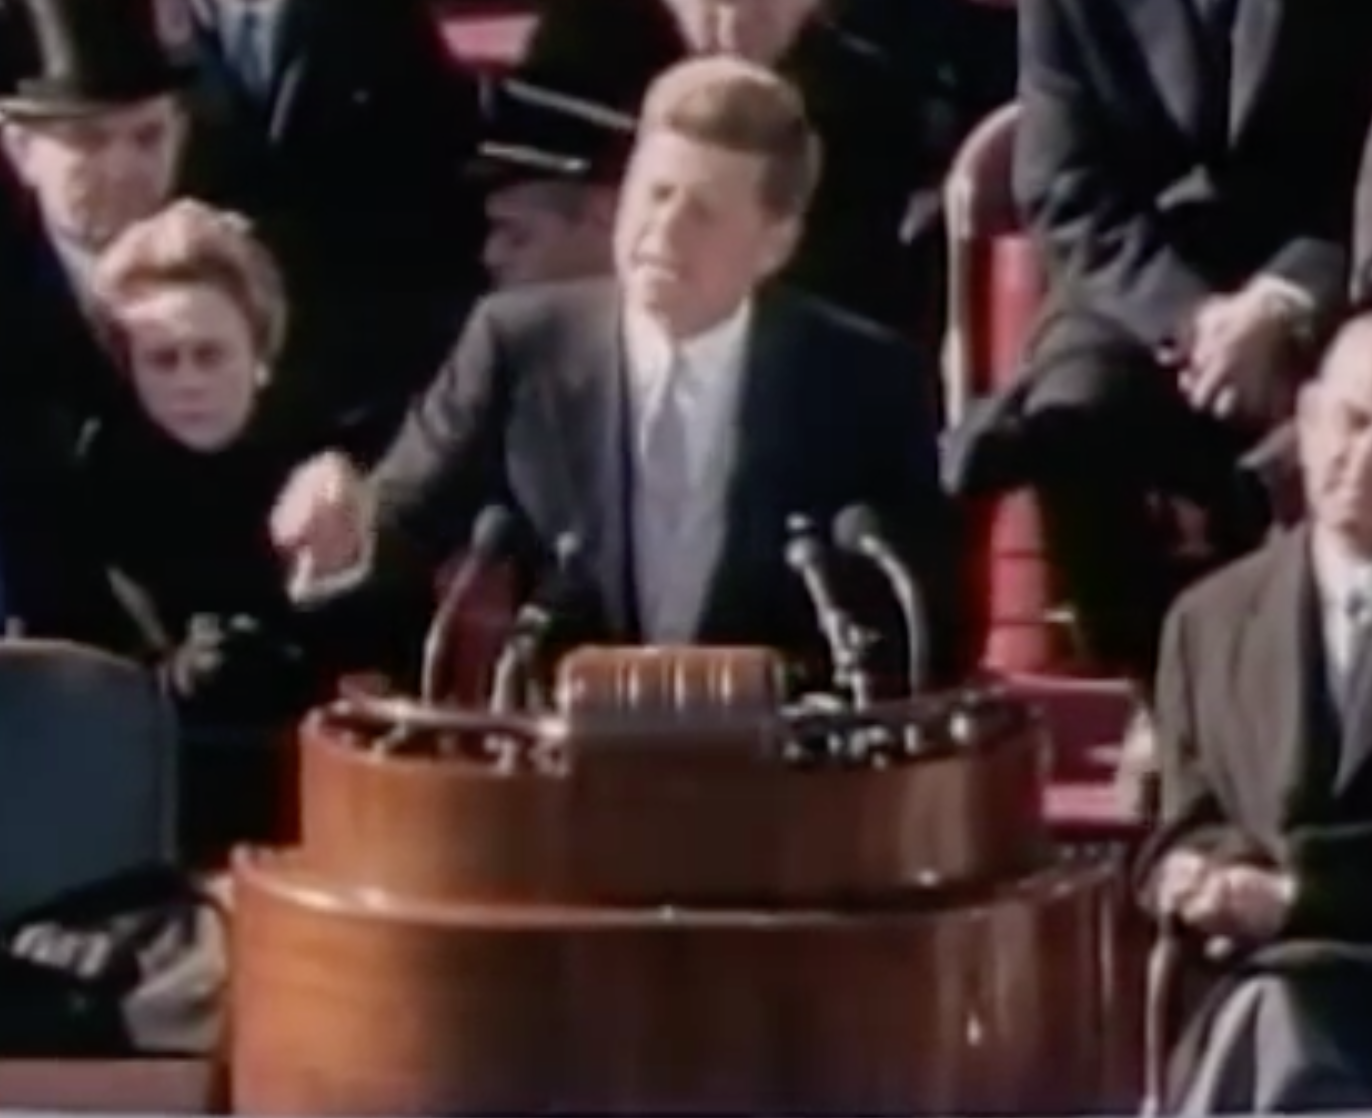
\includegraphics[width=0.8\textwidth]{./img/pastspeech.png}
  \caption[An example of past famous speech]{An example of past famous speech \protect\\
  (John F.Kennedy's Inaugural Adress in January 20, 1961)}
\label{fig:pastspeech}
\end{minipage}
\begin{minipage}[t]{0.35\textwidth}
\centering
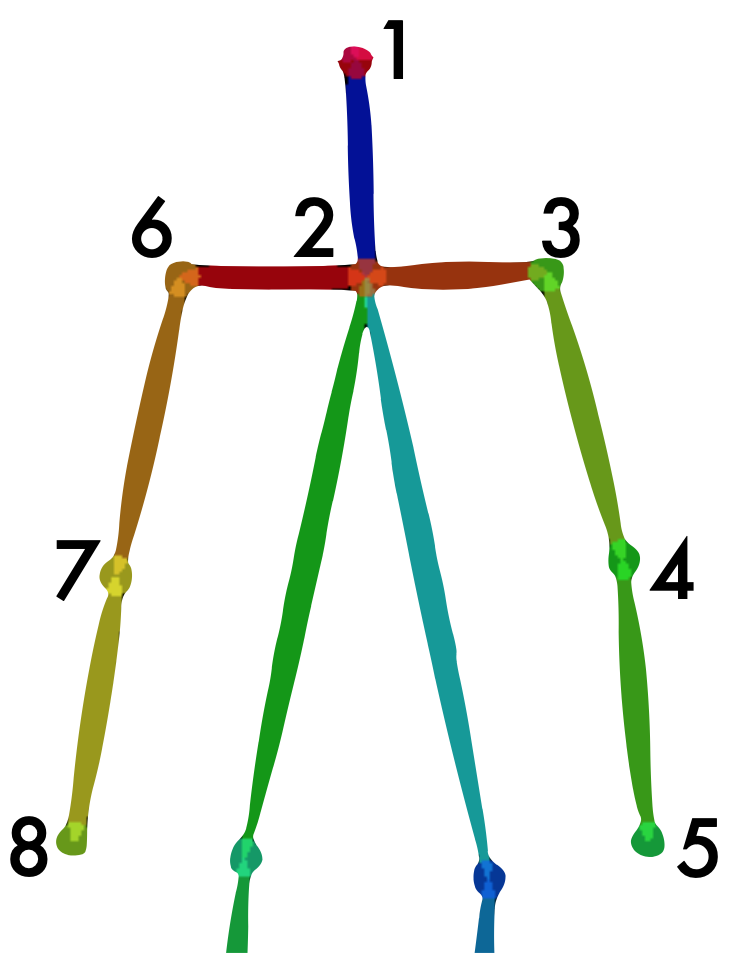
\includegraphics[width=0.8\textwidth]{./img/joint.png}
\caption{Extracted Joint}
\label{fig:joint}
\end{minipage}
\end{figure}

\subsection*{Extract Joint Data From Speech Video}

\par To train the presentation skill by imitating speech video, we need an appropriate video clip that should contain some gestures, proper vocal behaviors, and not too long. We watched some speech video and chose the famous \textit{We choose to go to the Moon} as our target video (Figure \ref{fig:wechosetogotothemoon}).


\munepsfig[width=0.7\textwidth]{wechosetogotothemoon}[Target speech video]{Speech video : \textit{We choose to go the Moon} (September 12,1962 in Rice Stadium )}

\par \textit{We choose to go to the Moon} is the famous tagline of a speech about the effort to reach the Moon delivered by President John F. Kennedy to a large crowd gathered attic Rice Stadium on September 12, 1962. The speech was intended to persuade the American people to support the Apollo program, the national effort to land a man on the Moon. In his speech, Kennedy characterized space as a new frontier, invoking the pioneer spirit that dominated American folklore. He infused the speech with a sense of urgency and destiny, and emphasized the freedom enjoyed by Americans to choose their destiny rather than have it chosen for them \cite{Affairs}. In this speech, he used gestures to stress his words and use some suitable pause to make his speech more impressive.

\par We cut the speech video into a short clip, which is 55 seconds, about 1654 frames. We download the source code of the OpenPose library from Github and compile it on a Linux desktop. Then we use the OpenPose library to extract joint data from target clip, and we will get a set of the processed image like figure \ref{fig:jfk}  and a set of JSON format data that contains the body joint of the orator like figure \ref{fig:json}.

\munepsfig[width=0.7\textwidth]{jfk}[An example of processed image]{An example of processed image}
%\munepsfig[width=0.5\textwidth]{json}[JSON format data example]{JSON format data example}

\par The Figure \ref{fig:json} shows the extracted data that contains the 18 kinds of joint. Each line contains the X coordinate, Y coordinate of each joint. The joint is ordered as table \ref{tab:jointorder}

\begin{figure}[!htbp]
  \begin{minipage}[b]{0.4\textwidth}
\centering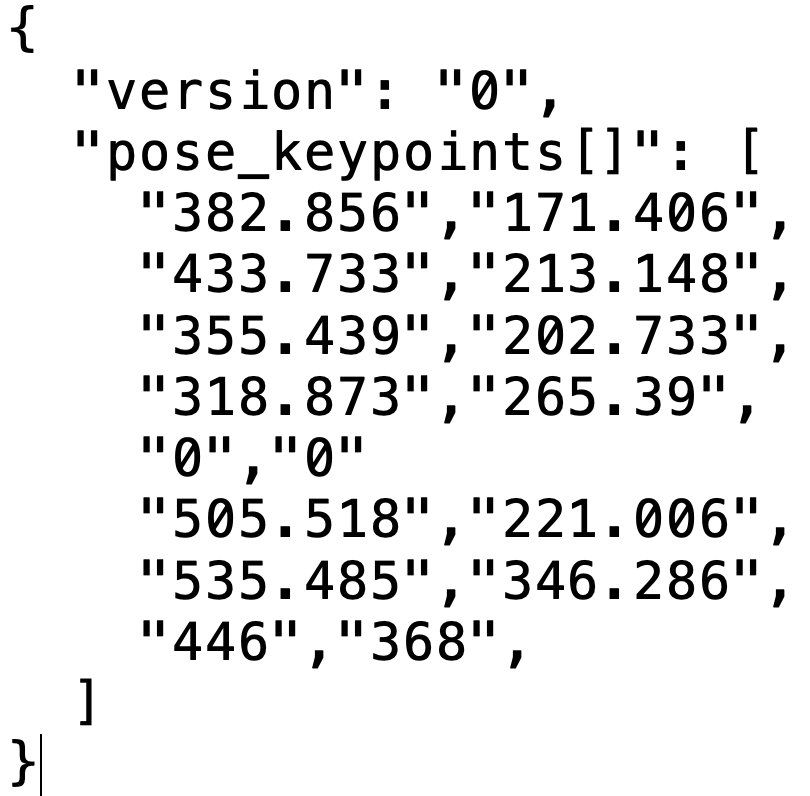
\includegraphics[width=0.75\textwidth]{./img/json.png}
  \caption{JSON format data example}
  \label{fig:json}
\end{minipage}
%\makeatletter\def\@captype{table}\makeatother
  \begin{minipage}[b]{0.6\textwidth}
\centering
\begin{tabular}{ll}
\hline
\# & Joint \\ \hline
1 & Head \\
2 & Neck \\
3 & Right shoulder \\
4 & Right wrist \\
5 & Right hand \\
6 & Left shoulder \\
7 & Left wrist \\
8 & Left hand \\ \hline
\end{tabular}
  \captionof{table}{Joint order}
  \label{tab:jointorder}
\end{minipage}
\end{figure}

\subsection*{Joint data editor}%
\label{sub:joint_data_editor}
\par However, OpenPose library can't detect some joint (see Figure \ref{fig:jfknohands}) or detect wrong joint (see Figure \ref{fig:jfkwrong}) sometimes due to the quality of speech clip and the effect of the podium.   

\begin{figure}[!htbp]
\centering
\begin{minipage}[t]{0.48\textwidth}
\centering
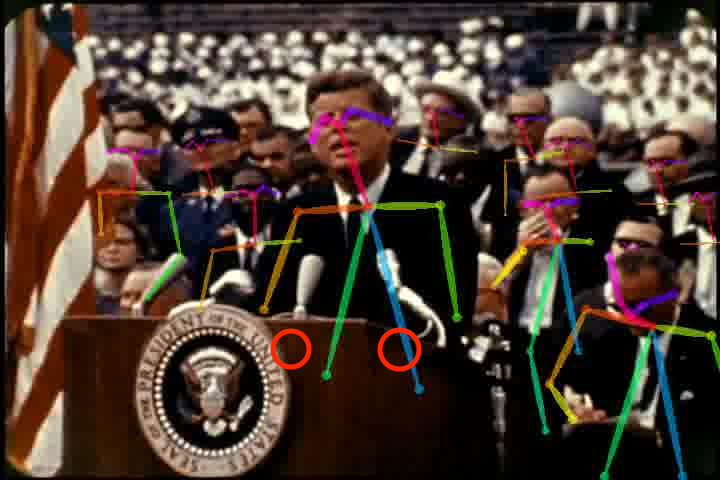
\includegraphics[width=0.85\textwidth]{./img/jfknohands.png}
\caption{An example of undetected joint}
\label{fig:jfknohands}
\end{minipage}
\begin{minipage}[t]{0.48\textwidth}
\centering
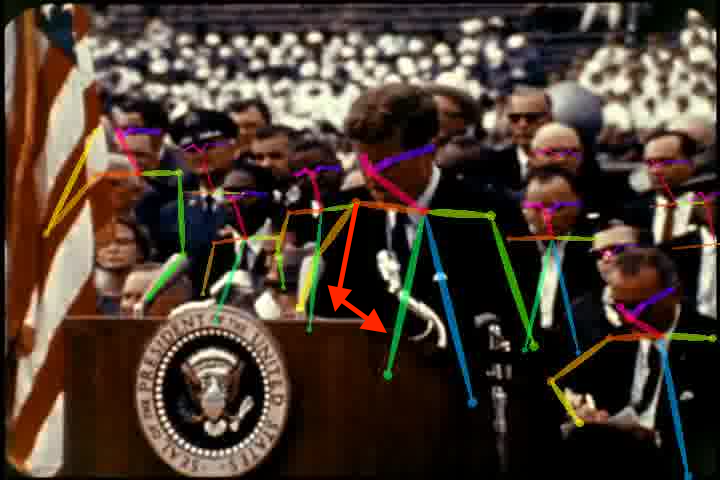
\includegraphics[width=0.85\textwidth]{./img/jfkwrong.png}
\caption{An example of wrongly detected joint}
\label{fig:jfkwrong}
\end{minipage}
\end{figure}
\par In the figure \ref{fig:jfknohands}, we can found that the OpenPose library can't detect the orator's hand (red circle) because of the orator is stand behind the podium. In the figure \ref{fig:jfkwrong}, we can find that the orator's right arm is detected wrongly due to the effect of the other people in the video, and the arm should be the position of red arrows. The selected video has 1654 frames, and we found that about half of all frames are not detected correctly.

\par To make the teacher data more accurate, we developed a joint data editor that can edit each joint data of each frame (Figure \ref{fig:jsoneditor}). This editor is wright by HTML and JavaScript and runs in the browser, and we can edit the joint data easily by it. At first, we need to click the joint name (such as RWrist in Figure \ref{fig:jsoneditor}) which is undetected or detected wrongly. Then, we need to click the selected joint's right position in the picture. Finally, we need to click the next button ($\longrightarrow$ in Figure \ref{fig:jsoneditor}), the joint data will be saved, and we can edit the next frame. 
\munepsfig[width=0.9\textwidth]{jsoneditor}[Joint data editor]{Joint data editor}

\par After edited all the frame, we will get a set of joint data. Then we will use those data as teacher data to do a template matching which will be introduced in section \ref{sec:template}.


\section{Extract Joint Data from Trainees}
\par To evaluate the trainee's speech and give trainee feedback in real-time. We also need to extract the trainee's joint data in real-time. Although the OpenPose library provides a method for real-time human key points extraction, it can only process about ten frames per second, and it isn't enough for real-time motion matching. 
\par To get trainees' joint data in real-time, we set up a Microsoft Kinect and employ Kinect for Windows SDK to extract joint data. The detail about Kinect was introduced in chapter \ref{chapter:preparation}. The Kinect can extract 25 kinds of joints information, and we only use the same 8 kinds of joints data (Fig \ref{fig:joint}) as OpenPose to decrease computational time. Although the Kinect camera can extract X, Y, Z coordinates of the joint, we only use X and Y coordinates because the OpenPose can only extract X and Y coordinates from the 2D video. 

\section{Evaluate Motion of Trainee}
\label{sec:template}
\par To evaluate how well does the trainee imitate past famous speech, we need to calculate the similarity of the trainee's motion and orator's motion in past speech. We employ a template matching algorithm to calculate the similarity. The joint data which extracted from past famous speech is called template data, and the joint data which extracted from the trainee's real-time video is called real-time data. The OpenPose library can extract 18 kinds of the key joint from a human and Kinect can extract 25 kinds of the key joint. However, we only use 8 kinds of key joint (see table \ref{tab:jointorder}). The correspondence of template data and real-time data is showed in Figure \ref{fig:jointmap}.

\munepsfig[width=0.9\textwidth]{jointmap}[Joint correspondence map]{Joint correspondence map}

\subsection*{Template Matching Alogrithm}
\par The traditional Euclidean distance based method allows calculating the Euclidean distance of past famous speech data and the real-time data to estimate the similarity. However, the Euclidean distance can't reflect the similarity reliably, and it's very sensitive to the position of the camera and noise. 
\par To estimate the similarity between the orator's motion in the past famous speech and the motion of trainees reliably, we calculate the cosine similarity of two adjacent limbs. The Figure \ref{fig:pipeline} and \ref{fig:pipeline2} shows the pipeline of the template matching algorithm. 

\munepsfig[width=0.9\textwidth]{pipeline}[The pipeline of template matching algorithm (part 1)]{The pipeline of template matching algorithm (part 1)}
\munepsfig[width=0.9\textwidth]{pipeline2}[The pipeline of template matching algorithm (part 2)]{The pipeline of template matching algorithm (part 2)}

\par Suppose that two adjacent joints' coordinate are ($X_{1}$,$Y_{1}$) and ($X_{2}$,$Y_{2}$), that limb vector will be:
\begin{equation}
    \bm {n}= \left (X_{1} , Y_{1}\right )-\left (X_{2} , Y_{2}\right )F
\label{vector}
\end{equation}
    
\par In accordance with the formula.\ref{vector}, we can get a assemble $\bm {P = (n_{1},n_{2},...n_{7})}$that include seven limbs' vectors (Figure \ref{fig:limbvector}).

\begin{figure}[!htbp]
\centering
\begin{minipage}[t]{0.45\textwidth}
\centering
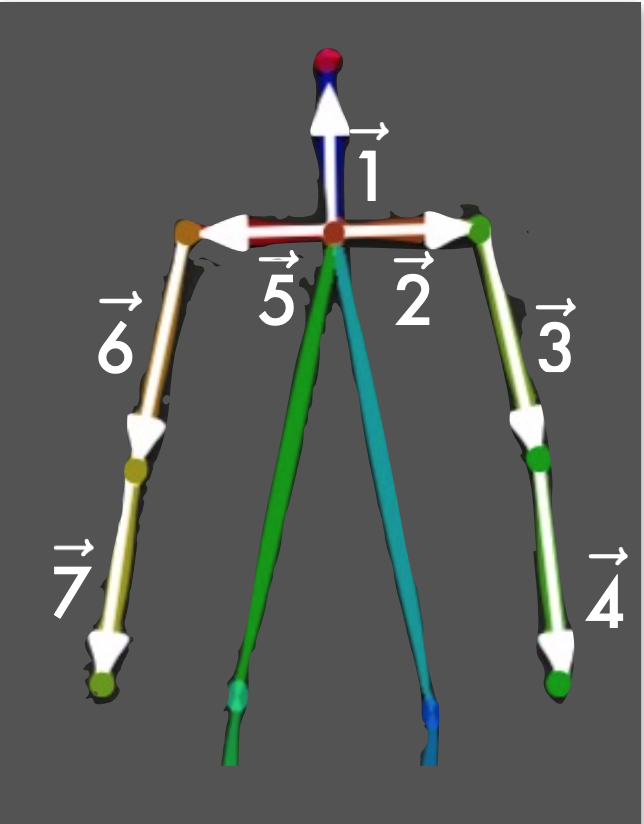
\includegraphics[width=0.85\textwidth]{./img/limbvector.png}
\caption{The vector of each limb}
\label{fig:limbvector}
\end{minipage}
\begin{minipage}[t]{0.51\textwidth}
\centering
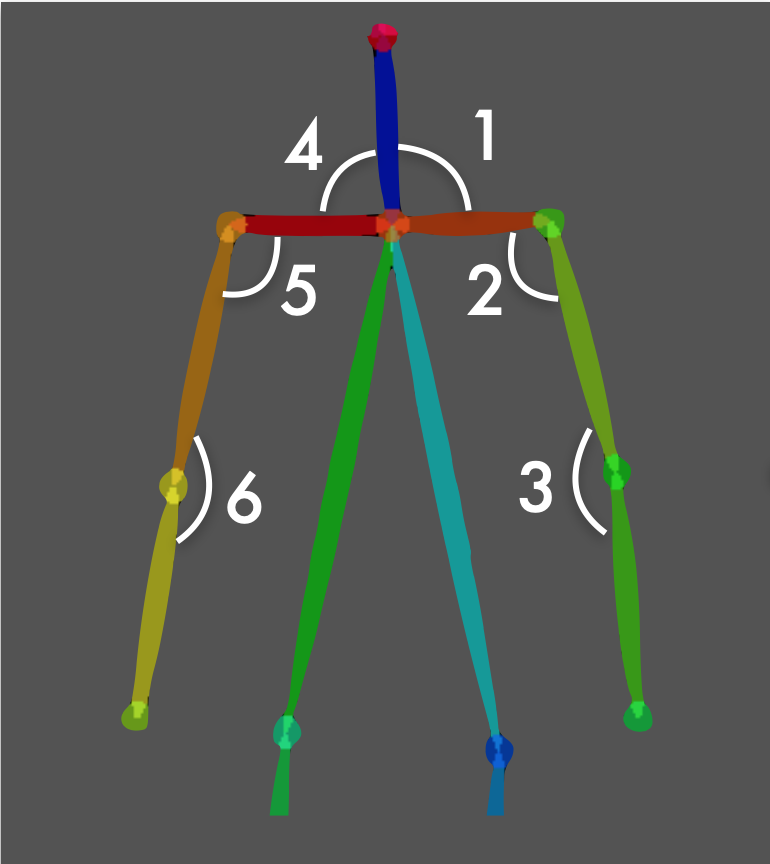
\includegraphics[width=0.85\textwidth]{./img/limbangle.png}
\caption{The angle of each two adjacent limbs.}
\label{fig:limbangle}
\end{minipage}
\end{figure}

\par Then calculate the cosine similarity of each two adjacent limb vectors A and B (eg. $A$ for $\vec 1$, $B$ for $\vec 2$ in Fig. \ref{fig:limbvector}) with the formula:
\begin{equation}
  \bm{cos} \ \bm{ \alpha_{i}} = \bm{\frac{\sum_{i =1}^{n}(A_{i}\times B_{i})}{\sqrt{\sum_{i=1}^{n}(A_{i})^{2}}\times \sqrt{\sum_{i=1}^{n}(B_{i})^{2}}}}
\label{cos}
\end{equation}
where $A_i$ and $B_i$ are components of vector $A$ and $B$ respectively.

\par Because each assemble $\bm{P}$ has 7 vectors, so we get a assemble $\bm{\theta_{template}}$ = $\lbrace\bm{\alpha_{t1}}$,$\bm{\alpha_{t2}}$,...$\bm{\alpha_{t6}}\rbrace$ that include six cosine similarity of each adjacent limbs (Figure \ref{fig:limbangle}) , which determine a motion template. In the same way, we can get a assemble $\bm{\theta_{real-time}}$ = $\lbrace\bm{\alpha_{r1}}$,$\bm{\alpha_{r2}}$,...$\bm{\alpha_{r6}}\rbrace$ with the joint data extracted by the Kinect that determine the real-time motion of trainee's body. 
\par Then calculate the difference of template motion and real-time motion by:
\begin{equation}
        \bm {\theta=\lbrace (\alpha_{r1}-\alpha_{t1}),(\alpha_{r2}-\alpha_{t2})...(\alpha_{r6}-\alpha_{t6})   \rbrace}
\label{difference}
\end{equation}
\par And the sum of cosine similarity difference will be:
\begin{equation}
\alpha _{sum} = \sum_{i=1}^{6}\alpha_{i}
\label{sum}
\end{equation}

\par The $\alpha_{i}$ represents the cosine similarity of different body parts, and the various parts' contribution for motion matching are diverse. For example, we wouldn't move our neck in a presentation, so the angle 1 (Figure \ref{fig:limbangle}) is always about 90$^\circ$, and it shouldn't affect obviously. In parallel, other bodies joint like hand or arm are always used to make some gesture in a presentation, so we should let it affect the score. Therefore we have to give each $\alpha_{i}$ a weight to compensate for the contribution's difference by:
\begin{equation}
  \omega_{i} = \frac{1-e^{-\frac{\alpha_{i}}{\alpha{sum}}}}{\sum_{i=1}^{6}(1-e^{-\frac{\alpha_{i}}{\alpha{sum}}})}    
\label{weight}
\end{equation}

\par According to the formula \ref{weight}, the large difference will have a high weight, and a light weight will be given to the insignificant difference (see the Weight in Figure \ref {fig:pipeline2}). Then we get a assemble $\bm{W}$ = $\lbrace \omega_{1},\omega_{2}...\omega_{6}\rbrace$, and the sum of $\bm{\omega_{i}}$ will be:

\begin{equation}
\bm{\sum_{i=1}^{6} \omega_{i}=1}
\end{equation}

\par For the difference of cosine similarity, the greater it is, the greater weight will be given. According to the difference of the adjacent limbs' angle and the weight, we can get a totalize as :
\begin{equation}
D = \sum_{i=1}^{6}\alpha_{i}\cdot\omega_{i}        
\label{differ}
\end{equation}
\par The totalize calculated by the formula.\ref{differ} can show the difference between real-time motion and template motion uniquely. And we normalize the totalize to a score between 0 and 100 by:
\begin{equation}
S = \begin{cases}
    (D_{std}-D)\cdot\frac{100-S_{std}}{D_{std}}+S_{std} &  0\leq D\leq D_{std} \\ 0&  D> D_{std} 
 \end{cases}
 \label{score}
\end{equation}

\par The range of matching degree score is 0-100. The greater the score $\bm{S}$ is, the real-time motion more similar to the template motion. In the formula \ref{score}, $\bm{D_{std}}$ is predetermined threshold for difference of angle, and the matching will be stringent if $\bm{D_{std}}$ is diminished. To avoid the negative number of score, the score will be set as 0 when $\bm{D<0}$. $\bm{S_{std}}$ is a predetermined parameter for controlling the score in the appropriate range. By several experiments, we set $\bm{D_{std}=60}$, $\bm{S_{std}=60}$ for best results. 

\section{System UI and Feedback for speech}
\par In training, we allow trainee imitate the past famous speech and the system calculate the similarity of trainee's motion and motion of orator in past famous speech. Then the trainee will get feedback about how well do they imitate. 
\munepsfig[width=0.7\textwidth]{systemui}[Prototype system UI]{Prototype system UI}
\par In our prototype system, we allow trainee watch their skeleton model, past speech video and score in real-time like Figure \ref{fig:systemui}. The score will update every second, and the trainee can adjust their motion to get a high score. The more similar the trainee imitating, the higher the score will be.

\newpage
\par We let some trainees try our prototype system and did a short interview. After the interview, we found that the trainee always looks at both the score and their skeleton model in training, so they can't focus on the speech. To solve this problem, we improved our system by connecting our system with a real-time visual feedback system like Figure \ref{fig:socket}.

\munepsfig[width=0.8\textwidth]{socket}[System structure]{System structure}


\newpage
\subsection*{Visual Feedback System \cite{YiHuang2018}}
\par The visual feedback system is an independent system build by Unity (see Figure \ref{fig:visualfeedback}). When the trainee wear an Oculus Rift (a kind of HMD), they can see a virtual hall and some virtual audiences. In the front of the virtual hall, there is a podium, and the past speech video will play over it. There are about 30 audiences, and when the trainee start imitating, the audiences will do different actions according to the score.
\munepsfig[width=0.9\textwidth]{visualfeedback}[Visual feedback]{Visual feedback \cite{YiHuang2018}}

